{
{\sffamily Dette afsnit vil præsentere vores resultater fra
eksperimentet, hvor vi har brugt den udvidede metode, til at vurdere
regionerne. Da eksperimentet blev kørt, har vi sat opløsningen på
regionernes approksimation med et gitter for højt, hvilket har
resulteret i, at vi kun har 524 brugbare resultater til rådighed. Dette
svare til $\mathsf{3.65\%}$ af de brugbare resultater fra den naive
kørsel. Vores datasæt bliver gennemgået alfabetisk efter kunstnerens
efternavn, så vi har kun resultater fra kunstnere med efternavn
startende med 'A' og 'B'.
}

\subsection{Håndtering af systematisk fejl}
Selvom denne analyse også har brugt den fejlbehæftede metode, til
udtrækning af regioner, så sorteres duplikater fra, når vi approksimerer
en region. Vi har gemt farven, som en region er blevet tildelt af
floodfill, og hvis denne farve ikke er at finde i regionens begrænsende
rektangel, betyder det, at regionen er blevet malet over senere. Vi
smider derfor denne region væk.

Den udvidede metode indeholder derfor ingen duplikater, men resultaterne
er ikke direkte sammenlignelige med dem fra den naive kørsel.

\subsection{Resultater}
Vi har i denne kørsel analyseret $608$ malerier, men som vist herunder i
udregning \ref{ud_tabel_fjern_detaljer}, har vi kun $524$ brugbare
resultater, når vi har fjernet de billeder, som ikke er hele malerier.
Dette svarer til en nedgang på $13.82\%$.

\begin{table}[H]
    \centering
    \begin{tabular}{r@{\ \ }p{12em}r|r@{.}l}
            & Analyserede malerier & $608$ & $100$ & $00\%$   \\
        $-$ & Udsnit af malerier   &  $84$ &  $13$ & $82\%$   \\\hline
            & Resultater           & $524$ &  $86$ & $18\%$
    \end{tabular}
    \caption[]{Udregning af brugbare resultater fra udvidet kørsel.}
    \label{ud_tabel_fjern_detaljer}
\end{table}

I udregning \ref{ud_tabel_fordeling} herunder undersøger vi, hvor mange
af de brugbare resultater, som har mindst en region liggende i det
gyldne snit. Vi har at der i $87.02\%$ af malerierne er blevet fundet
regioner i det gyldne snit, og vi kan derfor ikke afvise hypotese
\ref{hypo_binaer}.

\begin{table}[H]
    \centering
    \begin{tabular}{r@{\ \ }p{12em}r|r@{.}l}
            & Positive resultater   & $456$ &  $87$ & $02\%$ \\
        $+$ & Negative resultater   &  $68$ &  $12$ & $98\%$ \\\hline
            & Resultater i alt      & $524$ & $100$ & $00\%$
    \end{tabular}
    \caption[]{Et positivt resultat beskriver et maleri hvori der er
    fundet mindst en region i det gyldne snit, ved brug af den udvidede
    vurdering af regioner.}
    \label{ud_tabel_fordeling}
\end{table}

Fordelingen af regioner, over de fire gyldne snit i malerierne, ses i
udregning \ref{ud_tabel_fire_snit}. Intet af de fire snit afviger med
mere end $10\%$ fra et andet, og vi kan således ikke afvise hypotese
\ref{hypo_fire_g_snit}.

\begin{table}[H]
    \centering
    \begin{tabular}{r@{\ \ }p{12em}r|r@{.}l}
            & Regioner i snit 0   &  $405$ &  $22$ & $29\%$ \\
        $+$ & Regioner i snit 1   &  $421$ &  $23$ & $17\%$ \\
        $+$ & Regioner i snit 2   &  $499$ &  $27$ & $46\%$ \\
        $+$ & Regioner i snit 3   &  $492$ &  $27$ & $08\%$ \\\hline
            & Regioner i alt      & $1817$ & $100$ & $00\%$
    \end{tabular}
    \caption[]{Forholdet mellem de interessante regioner fundet i de
    fire gyldne snit ved udvidet vurdering.}
    \label{ud_tabel_fire_snit}
\end{table}

% Spacer! Ikke over denne linje HAHAHA

I graf \ref{antal_regioner_vertikale_cut_udvidet} er der afbilledet,
antale sammelet regioner i de 20 vertikale snit for helle datasættet.
Som man kan se er der fundet makant flere regioner i de to snit som
ligger tættest på miden, og færest ud i kanterne. 

\begin{figure}[h!]
	\begin{center}
		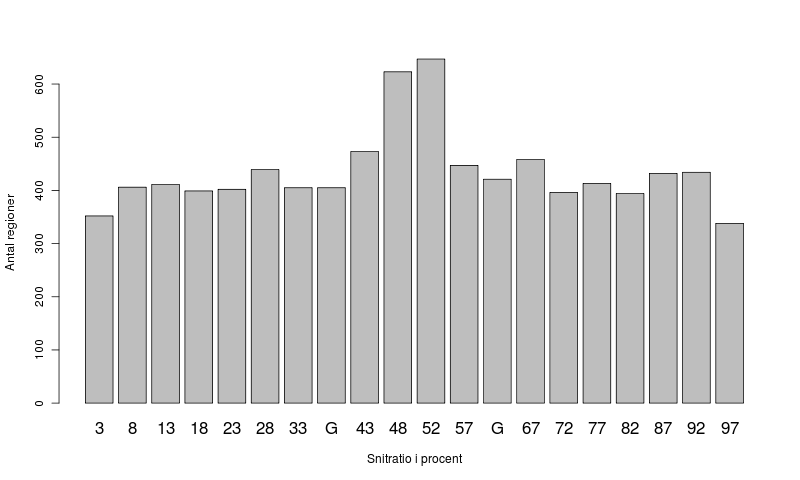
\includegraphics[width=0.9\textwidth]{afsnit/resultater/billeder/cut0cut1eatsperratioU.png}
	\end{center}
	\caption{Antal regioner i hvert af de 20 vertikale snit}
	\label{antal_regioner_vertikale_cut_udvidet}
\end{figure}

I graf \ref{antal_regioner_horisontale_cut_udvidet} er der samme
afbildning lavet, bare i det hoisontale plan, med venster side af grafen
svare til toppen af billedet. I denne graf er det 72,82 som peaker. Fra
52 og ned af, falder antal regioner gradvis. hvor i mod fra 52 og op gå
grafen lidt op og lidt ned. Kanterne er igen klart de lavest i grafen.

\begin{figure}[h!]
	\begin{center}
		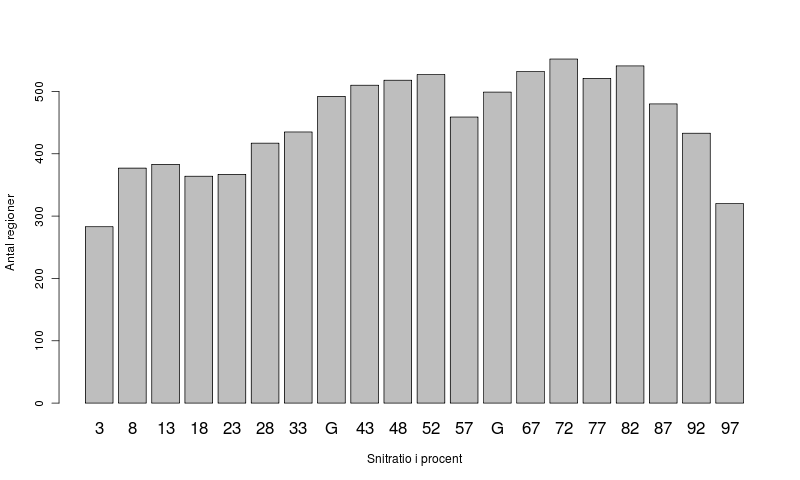
\includegraphics[width=0.9\textwidth]{afsnit/resultater/billeder/cut2cut3eatsperratioU.png}
	\end{center}
	\caption{Antal regioner i hvert af de 20 horisontale snit, hvor venstre side af grafen repræsentere øverst del af malerierne}
	\label{antal_regioner_horisontale_cut_udvidet}
\end{figure}

Ud fra disse observationer kan vi konkludere at der ikke er flere
regioner i det gyldne snit, en midden af billedet, og kan derfor
forkaste hypotese \ref{hypo_alle_andre_snit} og \ref{hypo_midten}.

I graf \ref{G_vs_to_trejedele_udvidet}, er de fire gyldne snit, samt
$\frac{2}{3}$ representeret. Som man kan se der ikke nogen entydighed på
hvad for et ration, der er dominerne, så vi kan forkaste hyptese
\ref{hypo_to_tredjedele}.

\begin{figure}[h!]
	\begin{center}
		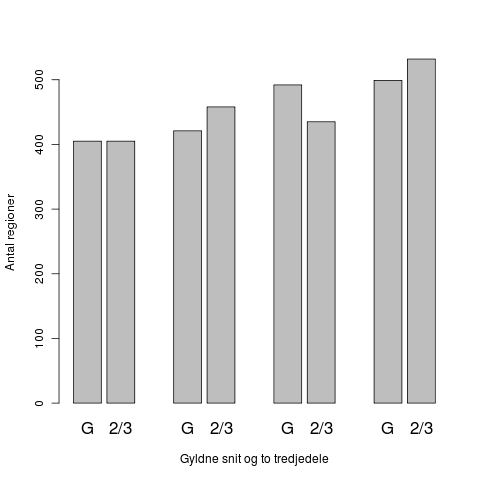
\includegraphics[width=0.6\textwidth]{afsnit/resultater/billeder/G_vs_to_tredjedeleU.png}
	\end{center}
	\caption{Procent vis antal regioner i de fire gyldne snit og deres tilhørene $\frac{2}{3}$ snit}
	\label{G_vs_to_trejedele_udvidet}
\end{figure}

\begin{table}[!h]
    \centering
    \begin{tabular}{|l|c|c|}
        \hline
            & Afvist & Ikke afvist  \\\hline
        1   &            & \checkmark   \\\hline
        2   &            & \checkmark   \\\hline
        3   & \checkmark$^{\textrm{*}}$ &              \\\hline
        4   & \checkmark &              \\\hline
        5   & \checkmark &    	\\\hline
        6   & \checkmark &              \\\hline
        7   &            &              \\\hline
        8   &            &              \\\hline
        9   &            & 	\\\hline
    \end{tabular}
    \caption[]{Hypoteser i forhold til den udvidet kørsel.
    $^{\textrm{*}}$Jvf. udregning \ref{tabel_real_dimensions}.
    }
    \label{hypoteser_udvidet}
\end{table}

} % Eh eh eh. Nallerne væk!

% vim: set tw=72 spell spelllang=da:
